\documentclass[letterpaper, 10 pt, conference]{ieeeconf}  % Comment this line out if you need a4paper
%\documentclass[a4paper, 10pt, conference]{ieeeconf}      % Use this line for a4 paper

%\IEEEoverridecommandlockouts                              % This command is only needed if 
                                                          % you want to use the \thanks command

\overrideIEEEmargins                                      % Needed to meet printer requirements.

% See the \addtolength command later in the file to balance the column lengths
% on the last page of the document

% The following packages can be found on http:\\www.ctan.org
%\usepackage{graphics} % for pdf, bitmapped graphics files
\usepackage{epsfig} % for postscript graphics files
%\usepackage{mathptmx} % assumes new font selection scheme installed
%\usepackage{times} % assumes new font selection scheme installed
%\usepackage{amssymb}  % assumes amsmath package installed
%\usepackage{epstopdf}

\usepackage{amsmath}		% assumes amsmath package installed
\usepackage{algorithm}
\usepackage{algpseudocode}
\usepackage{float}


\title{\LARGE \bf Monte Carlo PageRank Algorithm Implemented in Apache Spark}
%
% Single address.
% ---------------

\author{Sam Campbell \\  % <-this % stops a space
University of Waterloo \\
sj2campb@uwaterloo.ca
\thanks{$^{1}$ Sam Campbell is with the 
 School of Computer Science, University of Waterloo,
200 University Avenue, Waterloo, Ontario, Canada N2L 3G1.        {\tt\small }}%
}

%
% Single address.
% ---------------

\begin{document}

\maketitle
\thispagestyle{empty}
\pagestyle{empty}
%
\begin{abstract}
The PageRank algorithm has been a hotly researched topic, since its proven usefulness in high-profile applications. It calculates the relative importance of nodes in a directed graph based on the graph's link structure. The original method for calculating PageRank is called ``Power Iteration'', but it's not the only way to do it. A Monte Carlo approach can work as well, and that has been shown in other research over the last decade. A Monte Carlo approach allows for an easily updatable PageRank in an environment with a changing graph, but may sacrifice accuracy. This paper will investigate the accuracy of PageRank calculated using a Monte Carlo approach compared to the Power Iteration approach. The Monte Carlo algorithm takes as input a number of iterations and a number of random walks to perform, so this paper will also look at the optimal number of iterations and random walks to use.
\end{abstract}
%
\begin{keywords}
Monte Carlo, PageRank, Spark
\end{keywords}

%INTRODUCTION%
%=============%

\section{Introduction}
\label{sec:intro}
The PageRank algorithm has been widely used and researched since its introduction in 1998, due in part to its usefulness for ranking web pages at Google. Its purpose is to assign ``importance'' to nodes in a directed graph based on the graph's internal link structure. In the context of web pages, it assigns an importance score, or ``PageRank'' to pages. Pages with more links pointing to them tend to have a higher score, and pages that are pointed to by other ``important'' pages also tend to receive a higher score. PageRank values can be used for various applications, like ordering search results, browsing, estimating web site traffic, and many more graph-related applications.

The size of the entire web graph is very large and continues to grow, so for the PageRank algorithm to be effective, it should run as efficiently as possible. There are more than one ways to compute PageRank. Two of them are discussed in this paper: a Power Iteration (PI) approach and a Monte Carlo (MC) approach. The PageRank algorithm that was presented in 1998 by L. Page, S. Brin, R. Motwani, and T. Winograd \cite{Page99} uses the PI approach, which uses an iterative matrix-vector multiplication technique to calculate PageRank. A MC approach was introduced by K. Avrachenkov et al. in 2007 \cite{Avra07}. You can imagine the MC approach as a series of random walks through the graph, and the calculated PageRank for a node is relative to the number of times any walk visits that node.

Much research has gone into improving the performance of PageRank computation, though most research appears to be on improving the performance of the PI approach. More recently, research has gone into creating MC algorithms for distributed systems. Das Sarma et al. \cite{Sarma13} proposed an algorithm to calculate PageRank on a distributed system. In their research, they prove theoretically that one of their algorithms runs in $O(\log{n/E})$ number of rounds for directed or undirected graphs (like the web), and another runs in $O(\sqrt{log{n/E}})$ rounds for undirected graphs only. However, they did not have an implementation to test out their theoretical results. Another distributed Monte Carlo PageRank implementation was introduced by B. Bahmani et al. \cite{Bah11}, who described how a Monte Carlo random walk could be run in MapReduce with a minimal number of iterations. Their MapReduce algorithm is a more complicated calculation, but does have promise if it can effectively reduce the number of iterations. This paper will not investigate that algorithm, but will focus on the Monte Carlo algorithm compared to the Power Iteration algorithm.

The entire web graph is very large, so even with an efficient algorithm, PageRank may not be able to run very quickly, or at all on a single system. For example, the ClueWeb09 dataset contains the structure of the web from 2009. The dataset containing all unique URLs is 325GB uncompressed. One way to tackle the large dataset is to distribute the PageRank algorithm so that multiple computers are working on the calculation at once. This is where Apache Spark comes into play. It was built for fast cluster computing and large-scale data processing.

I've implemented a MC PageRank algorithm described by Das Sarma et al. \cite{Sarma13} in Spark. They devised two algorithms: Basic-PageRank-Algorithm and Improved-PageRank-Algorithm�. Only basic algorithm works for directed graphs like the web, so this paper will use that as the MC algorithm moving forward. I have also implemented a PageRank algorithm using the PI approach in Spark, and I'��ve compared the results. I'��ve specifically compared the convergence and accuracy of the PageRank vectors generated by the algorithms by looking at the PageRank of the 1st PageRank value, $\pi_1$ and 10th PageRank value, $\pi_{10}$.  to show how the PageRank distribution differs between the two approaches after a number of iterations.

%PAGERANK%
%==========%

\section{PageRank}
\label{sec:md}
A PageRank vector for a graph is defined as $\pi$�, where each element in $\pi$� represents the PageRank of a node in the graph.

%\subsection{Power Iteration PageRank}
The Power Iteration PageRank algorithm is based on the concept of a random web surfer, who is browsing web pages in a web graph. The surfer follows links on each page, but occasionally switches to a random page. This random jump is an important factor in the algorithm for mathematical reasons related to graph matrix properties, but also because it helps avoid pitfalls due to web pages that have no links to click on (dangling nodes). This random jump factor, denoted as $\epsilon$, is typically taken to be 0.15 \cite{Avra07, Page99}, meaning that 15\% of the time a surfer will jump to a random page, and the rest of the time they will click links. For more details on this algorithm, see the original paper \cite{Page99}.

%\subsection{Monte Carlo PageRank}
The random surfer model used in the original PageRank computation can also be represented by the MC approach using random walks. In this sense, a single surfer can be represented by one random walk $w_{ij}$, starting at node i and ending at node j. There is a probability, $\epsilon$, that the surfer will click away to a random page, so $(1-\epsilon)$ is the probability that they will follow an outgoing link from their current page. These basic rules can be used to guide the random walk. 

To describe one step in a random walk from node $i$, a random number would be generated. If the number is below $\epsilon$, then the walk ends. Otherwise, the walk picks one of the outgoing links with equal probability, which would be $1/n_O$, where $n_O$ is the number of outgoing links from the current page.

During a random walk, each node must record that it has been visited. The total number of visits to node $v$ is denoted by $\zeta_v$. The total number of visits over all nodes of all walks is $\frac{n K}{\epsilon}$. The PageRank for a node $v$, denoted as $\pi_v$, is estimated by dividing the number of visits to a node by the total number of all visits. The MC approach is naturally an approximation of the actual PageRank values, so an estimation of $\pi_v$ is denoted by $\tilde{\pi}_v$.

\begin{equation}
\tilde{\pi}_v = \frac{\zeta_v\epsilon}{n K}
\end{equation}

There are a few more important notations involved in the algorithm. $T_v^u$ is the number of random walks from $v$ to $u$ in a single iteration. $B$ is a constant used in calculating the number of iterations that the algorithm should run for to achieve an accurate result according to Das Sarma et al. \cite{Sarma13}: $B\log{n/\epsilon}$.
This algorithm is laid out by Das Sarma et al. in \cite{Sarma13}, and is summarized here in algorithm ~\ref{alg:BPR}.

% ALGORITHM %
%===========%
\begin{algorithm}

\caption{Basic-PageRank-Algorithm}
\label{alg:BPR}
\textbf{Input:} Number of nodes $n$ and reset probability $\epsilon$ \\
\textbf{Output:} PageRank of each node \\
\textbf{[Each node $v$ starts $K$ walks. All walks occur in parallel until they terminate. Termination probability for each walk is $\epsilon$, so the expected walk length is $1/\epsilon$ ]}

\begin{algorithmic}[1]
\State Each node $v$ maintains a count variable `$couponCount_v$' corresponding to number of random walk coupons held by $v$. Initially, `$couponCount_v = K$' for starting K random walks.

\State Each node $v$ also maintains a counter $\zeta_v$ for counting the number visits of random walks to it. Set $\zeta_v = K$ \\

\For{round $i = 1,2,...,B\log{n/\epsilon}$ } 
  \State Each node v holding at least one alive coupon (i.e., $couponCount_v \neq 0$) does the following in parallel:
  \State For every neighbour $u$ of $v$, set $T_u^v = 0$
  
  \For {j = 1,2,...,$couponCount_v$}
    \State With probability $1-\epsilon$, pick a uniformly random outgoing neighbour $u$
    \State $T_u^v := T_u^v + 1$
  \EndFor

\State Send the coupon counter number $T_u^v$ to the respective outgoing neighbours $u$.

\State Each node $u$ computes: $\zeta_u = \zeta_u + \sum_{v\in N(u)} {T_u^v}$
\State Update $couponCount_u = \sum_{v\in N(u)} {T_u^v}$

\EndFor \\
\State Each node $v$ outputs its PageRank as $\frac{\zeta_v\epsilon}{n K}$

\end{algorithmic}
\end{algorithm}

%IMPLEMENTATION%
%===============%

\section{Implementation}
Both the Power Iteration and Monte Carlo algorithms were implemented in Scala as Apache Spark jobs. Spark is a system designed for running large-scale distributed computations, and it abstracts the low-level details pertaining to managing the complexities of distributed computing. Similar to Hadoop's MapReduce, it brings the computation to where the data is stored. For instance, a large graph could be split up and stored across many servers. To run a Spark program on a distributed dataset, the program is passed to each Spark node, and executed on the node's portion of the dataset.

\subsection{Power Iteration Implementation}
The PI algorithm can be implemented in various ways, but one fairly intuitively way follows the random surfer notion. You can think of it as a method for distributing mass throughout the graph rather than many random walks, but the concept is not very different. To start, each node is given a starting ``mass'', which is $1/n$, where $n$ is the number of nodes in the graph. During each iteration, mass is distributed from each node through all of its outgoing links. If a node $i$ has $links_i$ outgoing links and currently contains mass $m_i$, then it distributes $\frac{m_i}{links_i}$ to each outgoing connected node. There are more details involved, like how to deal with nodes that have no outgoing links. For those details, refer to the original paper on PageRank \cite{Page99}.

\subsection{Monte Carlo Implementation}
To understand how this algorithm can be implemented in Spark, think of it in terms of a single random walk $w_{ij}$ that goes from node $i$ to node $j$. Only one step of every ongoing random walk can be carried out within one iteration. One iteration can be implemented using map and reduce functionality. The map stage figures out where walks will move to next, or if they will be discontinued. The output of the map stage is a series of destination node IDs paired with a walk count of 1. The reduce stage then sums up all the walks for each destination node, since there may be multiple walks visiting a node. The results of the reduce step is a one-to-one mapping of node IDs to their currently visiting walks. A further complication is that the total number of visits to each node must be incremented. This can be accomplished in Spark by combining the total visit counts with the visit counts for the latest walk step in various ways, such as a union or join function.

Spark fits together nicely with a distributed filesystem called HDFS, which allows for a graph to be distributed across computers in a cluster. For a walk $w_ij$, a small amount of information will have to be passed from node $i$ to node $j$. In a distributed graph, graph nodes $i$ and $j$ could be on separate computers. Spark handles this distribution of data in ``shuffle'' stages. Programmatically, this is done by outputting a key-value pair for each random walk after each iteration, where the key is the destination node ID for the next step of a walk, and the value is 1 for one walk. During a reduce function, spark executes a shuffle, that distributes these outputs to the proper computer in the cluster. After the shuffle step, each node is ready to calculate the next iteration of walk steps.

To figure out where a random walk will go next after node $j$, we need to find the outgoing nodes from $j$. Spark infrastructure handles the complicated distributed computing components of this operation by ensuring that this output gets joined back up with the link structure of node $j$, which may or may not be on a different computer in the cluster. An intuitive way to improve efficiency of any iterative algorithm like PageRank is to distribute the graph wisely, so that the fewest edges are broken when splitting the graph across computers.

%METHODS AND DATA%
%==================%
\section{Methods and Data}
Both PI and MC PageRank implementations were run against a simple graph dataset: the web graph of Stanford.edu from 2002. It is a directed graph consisting of 281,903 nodes, and 2,312,497 edges, and is a 31MB dataset when uncompressed. This dataset was used for the purpose of testing the convergence and accuracy of the two PageRank algorithms. It contains dangling nodes to ensure the implementations handle such a feature. Further work could expand upon this by using a much larger graph dataset. The advantage of an implementation in Spark comes when the graph dataset is too large to fit on one computer, or be processed by one computer. These Spark implementations should scale out to a clustered environment without the need to change any code.

%EXPERIMENT%
%===========%
\section{Experiment}
The focus of the experiment in this research was on the convergence and accuracy of the MC PageRank implementation compared to the PI PageRank implementation. In all results, the PageRank vector $\pi$ was in sorted order from highest to lowest, so let $\pi_i$ represent the PageRank ranked $i$ from the top.

Starting with the PI implementation, $\pi$ was calculated for the Stanford web graph by running the algorithm for 50 iterations. $\pi$ was recorded after 1, 3, 5, 10, 20, 30, and 50 iterations. Then, $\pi$ was calculated for the same dataset using the MC implementation. The MC implementation also requires a number of random walks to start with, so the series 1, 5, 10, 20, 30, 50 was used for that. There were 7 values of iterations used and 6 values of random walks, so in total the MC algorithm was run 42 times.

The analysis takes a somewhat similar approach to the analysis in \cite{Avra07}, in that I only look at one value of $\pi$ at a time for $\pi_1$ and $\pi_{10}$. While \cite{Avra07} compares different versions of MC algorithms, here I look at one MC algorithm over a varying number of random walks, and a varying number of iterations.


%OBSERVATIONS%
%=============%
\section{Observations}
There were a few interesting phenomena that appeared in the graphs of $\pi_1$ and $\pi_{10}$ when varying the number of iterations, as shown in Fig. 1 and Fig. 2 respectively. The most notable point is at 10 iterations. At this point, it is clear that the Power Iteration method is very close to its final converged value. This is the number of iterations where the MC estimation of $\pi_1$ is closest to the true value of $\pi_1$, but beyond this point, the MC estimated values continue to decrease. With a higher number of walks, the estimated value stays closer to the true value, whereas with only one walk per node, this dive is most drastic. Another interesting thing to note is that after just the first iteration of the MC algorithm, the initial values of $\pi_1$ are closer to the true value than the PI algorithm, with the exception of the single walk MC estimation. 

In the paper that introduces this algorithm \cite{Avra07}, they use 10 iterations of the MC algorithm without explaining why. This data suggests that is is the best number of iterations out of the samples tried here. Beyond that, it also suggests that after 10 iterations, the PageRank values may be less accurate. However, there should be more rigorous testing of this specific implementation and more data points to truly conclude whether or not this is the case.

\begin{figure}[H]
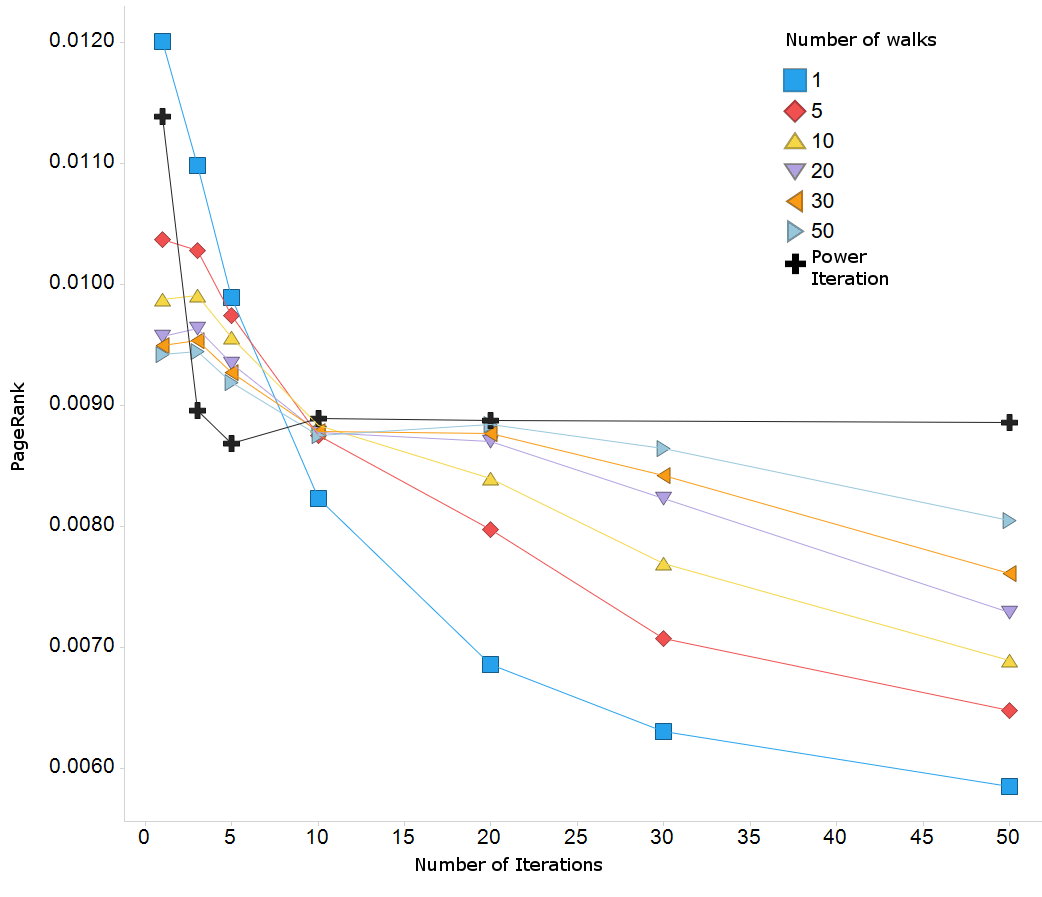
\includegraphics[height=7cm]{1st-Top-PageRank-vs-Number-of-Iterations-square}
\caption{ $\pi_1$ PageRank vs number of iterations. Each line represents a different number of walks.}
\label{fig:pi1-pr-vs-iterations}
\end{figure}

\begin{figure}[H]
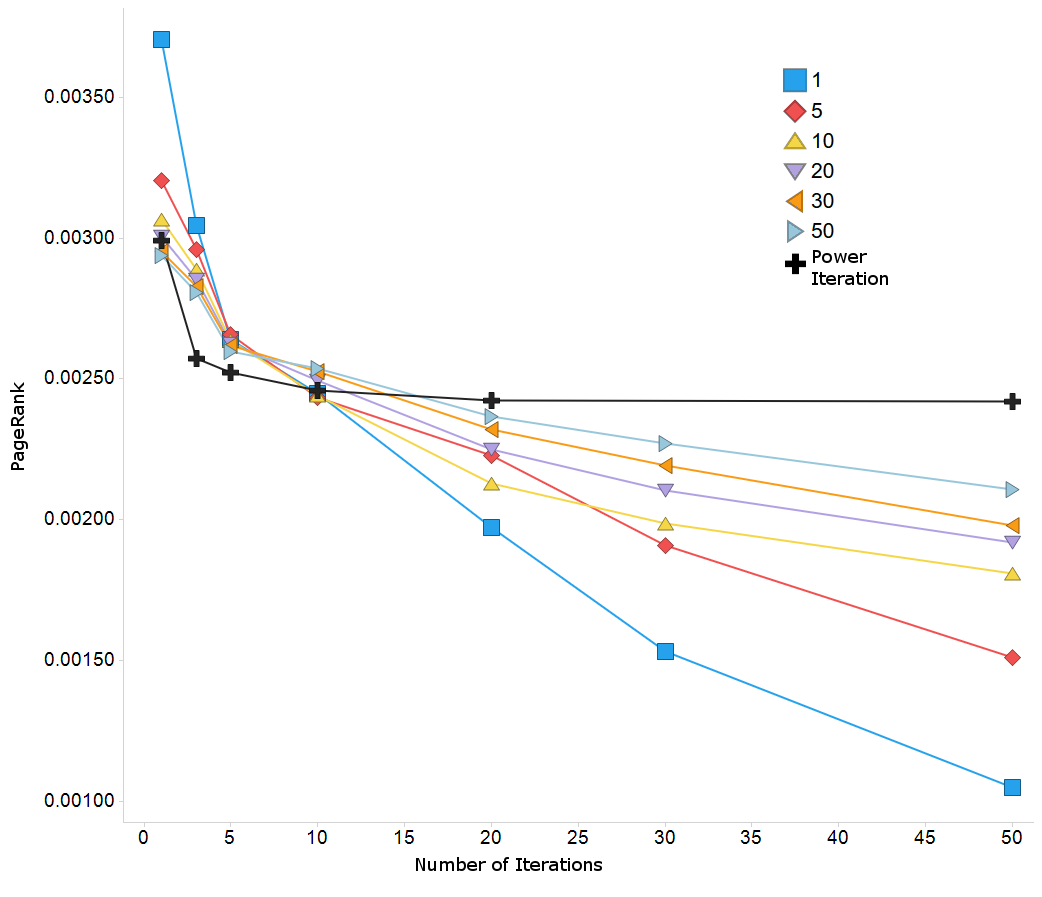
\includegraphics[height=7cm]{10th-Top-PageRank-vs-Number-of-Iterations-square}
\caption{ $\pi_{10}$ PageRank vs number of iterations.}
\label{fig:pi10-pr-vs-iterations}
\end{figure}

PageRank was also graphed against a varying number of walks for $\pi_1$ and $\pi_{10}$, as shown in Fig. 3 and Fig. 4. The horizontal dashed line represents the true values of $\pi_1$ and $\pi_{10}$, which were taken to be the values calculated by the Power Iteration method after 50 iterations. This data shows that more walks appear to increase convergence for all number of iterations. Also for both $\pi_1$ and $\pi_{10}$, when using fewer than 30 walks, 10 iterations is the most accurate, but with more than 30 walks, 20 iterations is more accurate.

\begin{figure}[H]
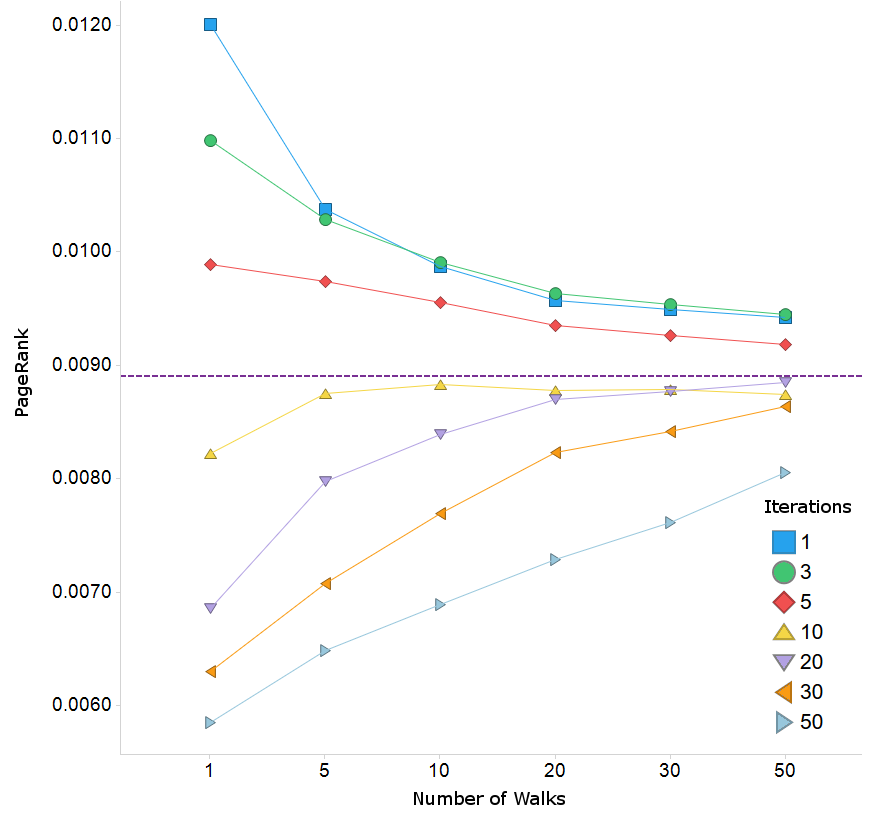
\includegraphics[height=7cm]{1st-Top-PageRank-vs-Number-of-Walks-square}
\caption{ $\pi_1$ PageRank vs number of walks. Each line represents a different number of iterations.}
\label{fig:pi1-pr-vs-walks}
\end{figure}

\begin{figure}[H]
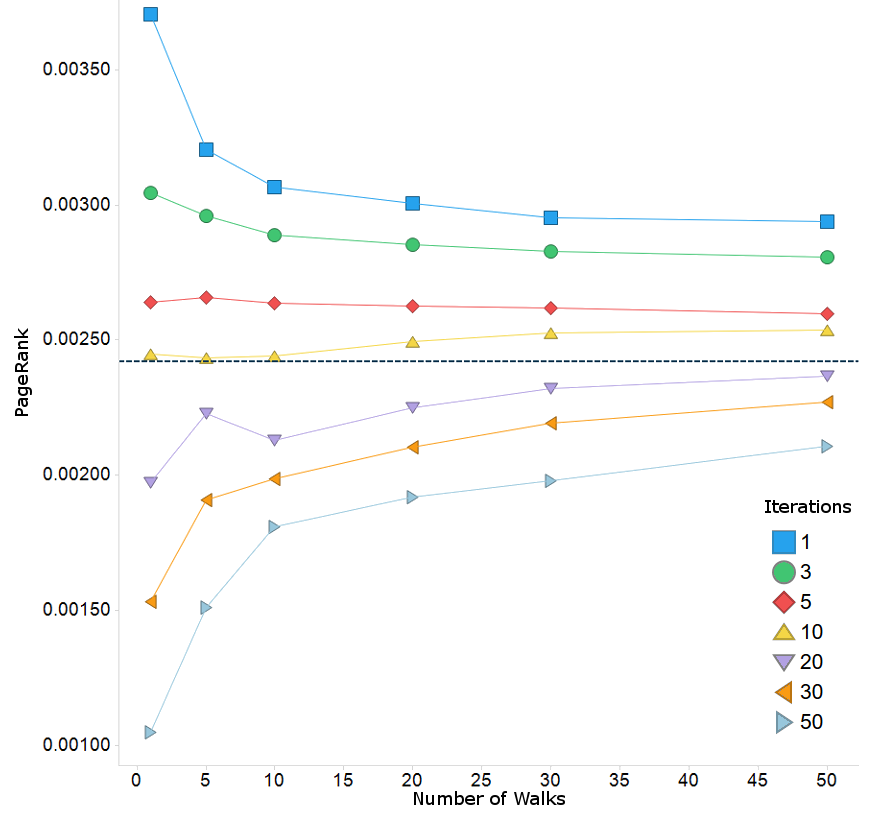
\includegraphics[height=7cm]{10th-Top-PageRank-vs-Number-of-Walks-square}
\caption{ $\pi_{10}$ PageRank vs number of walks.}
\label{fig:pi10-pr-vs-walks}
\end{figure}


%CONCLUSIONS%
%============%
\section{Conclusions}
The results showed a direct relationship between the number of walks used in the Monte Carlo algorithm and the accuracy of the calculated PageRank. This is an intuitive result, and the only reason for not using more walks is due to a balance of performance and accuracy. The relationship between the number of iterations and accuracy was more complicated. As the number of iterations increased up to 10, the MC PageRank calculations became very accurate and beyond 20 iterations, they continued to decrease away from the true PageRank value. Given this dataset and the measurements taken in this research, using 10 iterations would be the best solution for an accurate PageRank estimate using the Monte Carlo PageRank algorithm. Performance aside, using 50 walks (or more) would also help give the most accurate results.

Future work could investigate this approach on large-scale datasets and really put the Spark framework to use. On this small scale data set, performance comparisons were negligible, but further work could also determine how the PI and MC algorithms compare in terms of running-time performance.


%REFERENCES%
%============%
\bibliographystyle{IEEEbib}
\bibliography{McPageRankSpark}

\end{document}



